The journey set out from one clean theorem and followed it across sixteen variants, proving by hand what yielded to hand argument, building a machine where the proofs ran out, certifying the small cases the machine could close, and using the search to discover the dense graphs the proofs had singled out and to point at the ones still open. This closing chapter draws the threads together. It maps the directed frontier, where proof and certificate both still fall short of the full answer, names the two genuine surprises the landscape contains, gathers the sixteen answers into one picture, and says plainly what the program changed and where it stops.

\section{The directed frontier and the missing decomposition}

The directed arc problem is a race between a hub with $m(n-1)$ arcs and an augmented bipartite construction with $\floor{(n+m-2)^2/4}$ arcs (\Cref{const:directed-hub,const:augmented-bipartite}). They cross near $n=9$ at $m=3$, and \Cref{conj:dir-arc} asserts that their maximum is exact. Exhaustion proves the small $m=3$ cases, but the general upper bound is structural: it would follow if every non-hub extremiser admitted the complete $A\to B$ decomposition of \Cref{open:decomposition}. The difficult clause forbids arcs returning from $B$ to $A$, since one such arc lets routes escape through $A$ and defeats the internal $m-2$ budget. \Cref{fig:directed-frontier-pair} places the numerical crossover and that obstruction together.

% The crossover plot and the backward-arc diagram were side by side, which left
% the plot 2.8in wide against a 6.9in canvas and its axis labels at 3.5pt.
% Stacking them gives each most of the text width instead.
\begin{figure}[t]
    \centering
    \begin{subfigure}[b]{0.72\textwidth}
    \centering
    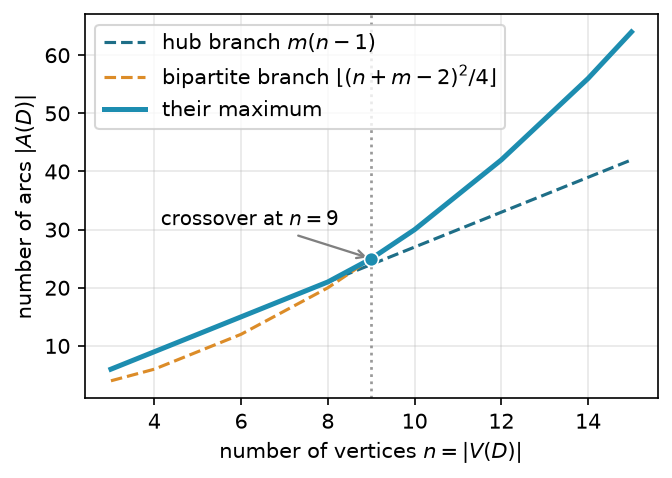
\includegraphics[width=\linewidth]{figures/directed_crossover.png}
    \caption{The two lower-bound branches at $m=3$.}
    \label{fig:crossover}
    \end{subfigure}

    \bigskip
    \begin{subfigure}[b]{0.72\textwidth}
\centering
\resizebox{\linewidth}{!}{%
\begin{tikzpicture}[>=Stealth, scale=0.92,
    abk/.style={gdirfaint},
    inb/.style={gdir, line width=1.3pt},
    back/.style={-{Stealth[length=2.3mm]}, line width=1.5pt, densely dashed, vertexred},
    esc/.style={-{Stealth[length=2.6mm]}, line width=2.1pt, vertexgreen!70!black}]
% ---------- panel (a): the clean A -> B structure ----------
\begin{scope}
  \node[smallvertex] (a1) at (0,1.0) {$a_1$};
  \node[smallvertex] (a2) at (0,-1.0) {$a_2$};
  \node[smallvertex] (b1) at (3,1.5) {$b_1$};
  \node[smallvertex] (b2) at (3,0) {$b_2$};
  \node[smallvertex] (b3) at (3,-1.5) {$b_3$};
  \node[font=\scriptsize, KULblauw1] at (0,2.4) {part $A$};
  \node[font=\scriptsize, KULblauw1] at (3,2.4) {part $B$};
  \foreach \x in {a1,a2}{\foreach \y in {b1,b2,b3}{\draw[abk] (\x) -- (\y);}}
  \draw[inb] (b1) to[bend left=20] (b2);
  \draw[inb] (b2) to[bend left=20] (b3);
  \node[font=\scriptsize, align=center] at (1.5,-2.5)
     {every arc $A\to B$, $B$ lightly\\thickened, none returns to $A$};
\end{scope}
% ---------- panel (b): one backward arc manufactures a route ----------
\begin{scope}[xshift=7.0cm]
  \node[smallvertex] (c1) at (0,1.0) {$a_1$};
  \node[smallvertex] (c2) at (0,-1.0) {$a_2$};
  \node[smallvertex] (d1) at (3,1.5) {$b_1$};
  \node[smallvertex] (d2) at (3,0) {$b_2$};
  \node[smallvertex] (d3) at (3,-1.5) {$b_3$};
  \foreach \x in {c1,c2}{\foreach \y in {d1,d2,d3}{\draw[abk] (\x) -- (\y);}}
  \draw[inb] (d1) to[bend left=20] (d2);
  \draw[inb] (d2) to[bend left=20] (d3);
  % backward arc b3 -> a1 (red), then the highlighted escape leg a1 -> b2 (green).
  % It bends downward (away from the green escape leg) to keep the two clear.
  \draw[back] (d3) to[bend left=28] (c1);
  \draw[esc] (c1) -- (d2);
  \node[vertexred, font=\scriptsize] at (1.35,-2.0) {backward arc $b_3\!\to\! a_1$};
  \node[font=\scriptsize, align=center] at (1.5,-2.5)
     {the route $b_3\to a_1\to b_2$\\now escapes $B$ through $A$};
\end{scope}
\end{tikzpicture}
}
\caption{Left, the desired $A\to B$ form. Right, one returning arc that breaks it.}
\label{fig:backward-arc}
    \end{subfigure}
\caption{The directed frontier in two views: the hub-to-wall crossover and the backward-arc obstruction to proving the wall optimal.}
\label{fig:directed-frontier-pair}
\end{figure}

The conjecture is nevertheless correct to first order and to the order of its error, and that much is a theorem with no hypothesis at all on the shape of the extremiser.

\begin{theorem}[The quadratic bound with a linear error]\label{thm:dir-arc-linear-error}
For all $m \ge 2$ and $n \ge 2$, every simple digraph $D$ on $n$ vertices with $\lec^{\max}_D \le m-1$ satisfies
\[
    |A(D)| \;\le\; \floorfrac{n^2}{4} \;+\; 4(m-1)(n-1),
\]
so for each fixed $m$,
\[
    \ell_m^{\mathrm{dir}}(n) \;=\; \frac{n^2}{4} \;+\; \Theta_m(n) \qquad (m\ge3),
\]
and, for $m\ge3$, both the leading constant $\tfrac14$ and the \emph{order} of the second-order term of \Cref{conj:dir-arc} hold unconditionally. At $m=2$, \Cref{thm:dir-arc-m2-exact} instead gives $\ell_2^{\mathrm{dir}}(n)=n^2/4+O(1)$ as $n\to\infty$.
\end{theorem}

The proof is in \Cref{app:proofs}. Its engine is a count of two-step routes: in a feasible digraph a vertex cannot have too many out-neighbours that reach one another, since the short detours through them would breach the ceiling, and that alone forces the arc count down to the wall plus a linear correction. What is left open is therefore only the coefficient of that linear term, somewhere between the conjectured $(m-2)/2$ and the proved $4(m-1)$. The next section takes up what the bound does and does not say about the \emph{shape} of an extremiser, which is a separate question answered by a cruder version of the same count.

The route family the count uses is internally vertex-disjoint and not merely arc-disjoint, which is what lets the whole argument be re-run under the stricter separation. Whitney's inequality alone would not justify the transfer, since it points the other way.

\begin{theorem}[Directed vertex problem, leading constant and order]\label{thm:dir-vertex-linear-error}
For all $m \ge 2$ and $n \ge 2$, every simple digraph $D$ on $n$ vertices with $\kap^{\max}_D \le m-1$ satisfies
\[
    |A(D)| \;\le\; \floorfrac{n^2}{4} \;+\; 4(m-1)(n-1),
\]
and consequently, for each fixed $m$,
\[
    k_m^{\mathrm{dir}}(n) \;=\; \frac{n^2}{4} \;+\; \Theta_m(n) \qquad (m\ge3).
\]
\end{theorem}

So the directed vertex problem, which \Cref{app:proofs} otherwise keeps carefully separate from the arc one, has the same leading term and the same order of error. Whether the two agree exactly for $m \ge 3$ is open.

Allowing parallel arcs, by contrast, closes the problem outright.

\begin{theorem}[Directed multigraph value, every $n$ and $m$]\label{thm:dir-multi-full}
For all $n \ge 2$ and $m \ge 2$,
\[
    L_m^{\mathrm{dir}}(n) \;=\; (m-1)\,M(n), \qquad M(n) := \max\!\Bigl(2(n-1),\ \floorfrac{n^2}{4}\Bigr).
\]
\end{theorem}

The extremisers include the doubled trees on the linear branch and the balanced one-way bipartite multigraph on the quadratic one. On the linear branch these are constructions exhibited rather than a classification, and \Cref{app:proofs} says explicitly that not every linear-branch extremiser has been classified. What makes the proof work, and what every earlier attempt lacked, is that it deletes a \emph{subgraph} at a time rather than a vertex. Inside any feasible multigraph there is a sparse skeleton that alone preserves which vertices reach which, and removing one copy of each of its arcs costs every pair at least one route. Peeling off $m-1$ such skeletons therefore accounts for every arc, and the parity obstruction that stopped the vertex-deletion induction never arises. Equality also classifies the quadratic extremisers once $n\ge\max(8,2m)$ (\Cref{thm:dir-multi-uniqueness}), and only the smaller range remains open.

\section{Two principal phenomena}

Across all the variation, two phenomena stand out as the ones a first guess would not have predicted.

The first is the divergence at $m = 5$. The edge and vertex problems agree for $m \le 4$, and it would be natural to expect them to agree forever. Instead they part company at the very next value, with $k_5(n) = \floor{8n/3} - 4$ for every $n \ge 6$ except the two sizes $n = 7$ and $n = 12$ that the paper settles separately, pulling strictly above $\ell_5(n)$ from $n = 14$ onwards (\Cref{thm:sorensen-thomassen}, and \Cref{rem:threshold-convention} for the counting convention that fixes the constant). The separation is genuinely a fact about $m$ rather than about $n$: at $m = 5$ the two values still agree at every size up to $n = 13$ and only then come apart, and beyond $m = 5$ the vertex problem becomes genuinely hard and has stayed open since 1974.

The second is the quadratic bipartite phenomenon. In an undirected graph every edge contributes to the degree of both its endpoints, and Mader's theorem turns that symmetry into a hard ceiling of $\floor{m(n-1)/2}$ edges, linear in $n$. A digraph breaks the symmetry. The one-directional wall of \Cref{const:bipartite} sends every arc from one half of the vertices to the other and holds $\floor{n^2/4}$ of them at $\lambda^{\max} = 1$, because a route must cross the wall exactly once and nothing crosses back to offer a second. An arc count growing like $n^2$ while the connectivity stays at one is something no undirected graph can do past a handful of vertices, and it is why the initial linear conjecture for the directed case fails already at $m = 2$, where on $n = 8$ the wall holds $16$ arcs against the hub's $14$. \Cref{const:augmented-bipartite} carries the same idea to every $m$ by letting each vertex of the larger part absorb $m - 2$ extra in-arcs from inside that part, which buys $m - 2$ short detours per pair and lifts $\lambda^{\max}$ to $m - 1$ while the count climbs to $\floor{(n+m-2)^2/4}$. Its $m = 3$, $n = 10$ instance holds thirty arcs against the naive prediction of twenty-seven.

The quadratic term is what makes the directed cases the deepest in the thesis. The upper bound argument must explain why no configuration beats the bipartite wall, which requires producing the partition in the first place, ruling out backward arcs, and controlling the internal structure of the large part $B$. That structural task is exactly what \Cref{open:decomposition} has not yet resolved for $m \ge 3$. What \Cref{prop:dir-arc-stability} and \Cref{thm:dir-arc-linear-error} show is that the wall is at least the right shape, and the two say it in different currencies, which is worth keeping apart. In \emph{size}, the extremal value lies within $O_m(n)$ of the wall's count, so the difficulty is a constant inside the second-order term rather than the phenomenon. In \emph{shape}, every feasible digraph becomes a subgraph of a one-directional bipartite graph after deleting $O(\sqrt{m}\,n^{3/2})$ arcs, which is a weaker error term because it comes from the cruder of the two counts, the one that does not get to induct on a low-degree vertex. The undirected problem has no analogous obstacle, because Mader's degree-counting argument closes it in a few lines. The quadratic phenomenon is therefore not just a curiosity: it is the geometric reason the directed and undirected problems live on different levels of difficulty.

\section{Summary of the sixteen variants}

\Cref{tab:summary} records the status of all sixteen structural variants. Each entry is marked by how it is known: proved by hand here or in \Cref{app:proofs}, cited to the literature, conjectured with a proved lower bound, or, for the two rows where only the leading term is settled, proved asymptotically. No row now rests on a machine certificate alone. That category was live in earlier drafts, when the directed multigraph value was known only for the sizes the cut-counting optimisation could close, and \Cref{thm:dir-multi-full} retired it. The distinction is the honesty contract of \Cref{ch:machine} carried through to the summary. \Cref{fig:variant-tree-status} shows the same distinction as a picture before the table spells out every case.

\begin{figure}[t]
\centering
\resizebox{\textwidth}{!}{%
\begin{tikzpicture}
  \node[vtroot, fill=KULblauw3a!18]  (root) at (9.0,3.9) {Problem 915};
  \node[vtmodel, fill=KULblauw3a!12] (simple) at (1.8,2.6)  {simple};
  \node[vtmodel, fill=KULblauw3a!12] (multi)  at (6.6,2.6)  {multi};
  \node[vtmodel, fill=KULblauw3a!12] (hyper)  at (11.4,2.6) {hyper};
  \node[vtmodel, fill=KULblauw3a!12] (mhyper) at (16.2,2.6) {multi-hyper};
  \draw[vtedge] (root) -- (simple);
  \draw[vtedge] (root) -- (multi);
  \draw[vtedge] (root) -- (hyper);
  \draw[vtedge] (root) -- (mhyper);
  \node[vtdir, fill=regimeProved!22]      (d0) at (0.6,1.3)  {undirected};
  \node[vtdir, fill=regimeConjectured!22] (d1) at (3.0,1.3)  {directed};
  \node[vtdir, fill=regimeProved!22]      (d2) at (5.4,1.3)  {undirected};
  \node[vtdir, fill=regimeConjectured!22] (d3) at (7.8,1.3)  {directed};
  \node[vtdir, fill=regimeProved!22]      (d4) at (10.2,1.3) {undirected};
  \node[vtdir, fill=regimeOpen!28]        (d5) at (12.6,1.3) {directed};
  \node[vtdir, fill=regimeProved!22]      (d6) at (15.0,1.3) {undirected};
  \node[vtdir, fill=regimeOpen!28]        (d7) at (17.4,1.3) {directed};
  \draw[vtedge] (simple) -- (d0);
  \draw[vtedge] (simple) -- (d1);
  \draw[vtedge] (multi)  -- (d2);
  \draw[vtedge] (multi)  -- (d3);
  \draw[vtedge] (hyper)  -- (d4);
  \draw[vtedge] (hyper)  -- (d5);
  \draw[vtedge] (mhyper) -- (d6);
  \draw[vtedge] (mhyper) -- (d7);
  \node[vtleaf, fill=regimeProved!16]      (l0)  at (0,0)    {edge};
  \node[vtleaf, fill=regimeProved!16]      (l1)  at (1.2,0)  {vertex};
  \node[vtleaf, fill=regimeConjectured!16] (l2)  at (2.4,0)  {edge};
  \node[vtleaf, fill=regimeConjectured!16] (l3)  at (3.6,0)  {vertex};
  \node[vtleaf, fill=regimeProved!16]      (l4)  at (4.8,0)  {edge};
  \node[vtleaf, fill=regimeProved!16]      (l5)  at (6.0,0)  {vertex};
  \node[vtleaf, fill=regimeProved!16]      (l6)  at (7.2,0)  {edge};
  \node[vtleaf, fill=regimeConjectured!16] (l7)  at (8.4,0)  {vertex};
  \node[vtleaf, fill=regimeProved!16]      (l8)  at (9.6,0)  {edge};
  \node[vtleaf, fill=regimeProved!16]      (l9)  at (10.8,0) {vertex};
  \node[vtleaf, fill=regimeOpen!22]        (l10) at (12.0,0) {edge};
  \node[vtleaf, fill=regimeOpen!22]        (l11) at (13.2,0) {vertex};
  \node[vtleaf, fill=regimeProved!16]      (l12) at (14.4,0) {edge};
  \node[vtleaf, fill=regimeProved!16]      (l13) at (15.6,0) {vertex};
  \node[vtleaf, fill=regimeOpen!22]        (l14) at (16.8,0) {edge};
  \node[vtleaf, fill=regimeOpen!22]        (l15) at (18.0,0) {vertex};
  \draw[vtedge] (d0) -- (l0);  \draw[vtedge] (d0) -- (l1);
  \draw[vtedge] (d1) -- (l2);  \draw[vtedge] (d1) -- (l3);
  \draw[vtedge] (d2) -- (l4);  \draw[vtedge] (d2) -- (l5);
  \draw[vtedge] (d3) -- (l6);  \draw[vtedge] (d3) -- (l7);
  \draw[vtedge] (d4) -- (l8);  \draw[vtedge] (d4) -- (l9);
  \draw[vtedge] (d5) -- (l10); \draw[vtedge] (d5) -- (l11);
  \draw[vtedge] (d6) -- (l12); \draw[vtedge] (d6) -- (l13);
  \draw[vtedge] (d7) -- (l14); \draw[vtedge] (d7) -- (l15);
  \node[vtleaf, fill=regimeProved!16, minimum width=8mm]      (leg1) at (0,-1.3) {};
  \node[anchor=west, font=\scriptsize] at (0.9,-1.3) {closed form proved, with exceptions in \Cref{tab:summary}};
  \node[vtleaf, fill=regimeConjectured!16, minimum width=8mm] (leg2) at (0,-2.1) {};
  \node[anchor=west, font=\scriptsize] at (0.9,-2.1) {conjectured, matching certified small $n$};
  \node[vtleaf, fill=regimeOpen!22, minimum width=8mm]        (leg3) at (0,-2.9) {};
  \node[anchor=west, font=\scriptsize] at (0.9,-2.9) {leading constant proved, exact value open};
\end{tikzpicture}%
}
\caption{Status of the sixteen variants. Blue marks a proved closed form in the ranges stated in \Cref{tab:summary}, red a conjectured exact formula with proved lower bound, and amber a proved leading term with unknown exact value. The table is authoritative for exceptions and conventions.}
\label{fig:variant-tree-status}
\end{figure}

\begin{table}[htbp]
\centering
\renewcommand{\arraystretch}{1.06}
\setlength{\tabcolsep}{4pt}
\begin{tabularx}{\textwidth}{@{}>{\raggedright\arraybackslash}p{0.155\textwidth}XX@{}}
\toprule
Model & Edge/arc-disjoint & Vertex-disjoint \\
\midrule
undirected simple graph
  & $\floor{m(n-1)/2}$, exact
  & edge value for $m\le4$, $\floor{8n/3}-4$ for $m=5$, $n\ne7,12$, open for $m\ge6$ \\
undirected multigraph
  & $(m-1)(n-1)$, exact
  & simple value, adjacency-count convention \\
undirected $r$-hyper, simple
  & $\le\floor{(m-1)(n-1)/(r-1)}$, equality when $r\ge3$ and $m-1\le\binom{n-2}{r-2}$
  & $\floor{(n-1)/(r-1)}$ for $m=2$, $\le\floor{2(n-1)/(r-1)}$ for $m=3$, same equality range \\
undirected $r$-hyper, multi
  & the same bound, equality when $(r-1)\mid(n-1)$
  & the same bounds, with repeats never helping at $m=2$ and closing cases the simple model misses at $m=3$ \\
directed simple graph
  & $M(n)$ for $m=2$, $n^2/4+\Theta_m(n)$ for $m\ge3$, exact then conjectured
  & $M(n)$ for $m=2$, $n^2/4+\Theta_m(n)$ for $m\ge3$, exact equality with the arc value open \\
directed multigraph
  & $(m-1)M(n)$, exact
  & simple-digraph value, adjacency-count convention \\
directed $r$-hyper, simple
  & $(1+o(1))(m-1)n^2/[4(r-1)]$ for fixed $r,m$, leading term exact
  & same leading term for fixed $r,m$ \\
directed $r$-hyper, multi
  & same leading term, the bound being proved for multihypergraphs
  & same leading term for fixed $r,m$ \\
\bottomrule
\end{tabularx}
\caption{The sixteen variants and the strongest result known for each.}
\label{tab:summary}
\end{table}

Here $M(n)=\max(2(n-1),\floor{n^2/4})$. Simple-graph formulas assume
$n\ge m$. Below that range the complete object gives the trivial maximum.
The edge-hypergraph bound is attained when $(r-1)\mid(n-1)$ for
multihypergraphs, and for simple hypergraphs when $r\ge3$ and
$m-1\le\binom{n-2}{r-2}$. The $m=3$ vertex-hypergraph bound is attained when
$r\ge3$ and $2\le\binom{n-2}{r-2}$. The two multigraph vertex rows use the
counting convention of \Cref{sec:parallel-convention}. Under the other
convention, where parallel copies count as distinct routes, the multigraph
vertex question becomes a separate extremal problem, studied in
\Cref{sec:multi-vertex-standard} and listed among the open problems below. Full statements and
exceptions are in \Cref{thm:mader,thm:leonard,thm:sorensen-thomassen,prop:hyper-edge,thm:simple-hyper-edge,thm:hyper-vertex-m2,thm:hyper-vertex-m3,thm:dir-multi-full,thm:dir-arc-linear-error,thm:dir-vertex-linear-error,thm:dir-hyper-constant}.

\subsection{Orientation models for the directed hypergraph}
\label{sec:orientation-models}

The directed hypergraph row of \Cref{tab:summary} rests on one bound, which pins the leading term where previously only a factor-of-four window was known.

\begin{theorem}[The directed hypergraph constant]\label{thm:dir-hyper-constant}
Let $r \ge 2$ and $m \ge 2$. Every forward directed $r$-uniform multihypergraph
$\HH$ on $n \ge 2$ vertices with $\kap^{\max}_{\HH} \le m-1$ satisfies
\[
    |E(\HH)| \;\le\; \frac{m-1}{r-1}\floorfrac{n^2}{4} \;+\; 4(m-1)^2 (n-1).
\]
The same bound therefore holds under $\lec^{\max}_{\HH} \le m-1$, which is the
stronger hypothesis by $\kap \le \lec$. Hence for fixed $r$ and $m$ both the
edge- and the vertex-disjoint maxima are
$\bigl(1+o(1)\bigr)(m-1)n^2/\bigl(4(r-1)\bigr)$, and the bipartite construction
of \Cref{prop:dir-hyper-first} is asymptotically optimal for both.
\end{theorem}

The proof, in \Cref{app:proofs}, forms the one-step shadow digraph whose arc
$u\to v$ records that some hyperedge has tail $u$ and head $v$.  A matching
argument transfers the hypergraph route ceiling to the shadow's two-step route
budget, after which \Cref{lem:two-step-budget} controls the shadow and a
tail--head incidence count converts its arcs back to hyperedges. Since the
bipartite construction already attains that leading term, it is asymptotically
optimal.

The table uses the \emph{forward} convention of one tail and $r-1$ heads. More generally a hyperedge may split into non-empty tail and head sets. Reversal makes the one-head \emph{backward} model exactly equivalent to forward (\Cref{lem:dir-hyper-duality}), while \Cref{thm:dir-hyper-general-constant} proves that arbitrary splits share the same leading term under both separations. Thus the orientation choice does not add another asymptotic row to \Cref{tab:summary}.

Finite values may differ when vertices are scarce. Whether forward and general
agree exactly once $n>r$ remains open, and the thesis uses the forward convention
throughout its sixteen-variant summary.

\subsection{The multigraph vertex problem under the other convention}
\label{sec:multi-vertex-summary}

One variant of \Cref{tab:summary} deserves a statement of its own, because it is the one place where a whole extremal problem turns out to be a packing problem in disguise. Under the convention that parallel copies count as distinct routes, the multigraph vertex question becomes a genuinely different problem, written $K_m^{\mathrm{multi}}(n)$ and studied in \Cref{sec:multi-vertex-standard}. Its answer is additive over the blocks of the underlying simple graph, because adjacent vertices always share a block and no route between them ever leaves it.

\begin{theorem}[The multigraph vertex problem is a knapsack over blocks]\label{thm:multi-vertex-blocks}
For a $2$-connected graph $B$, or a single edge, write
\[
    g_m(b) \;:=\; \max\bigl\{\, W_m(B) \;:\; B \text{ $2$-connected or an edge, } |V(B)| = b,\ \kap^{\max}_B \le m-1 \,\bigr\} ,
\]
with $g_m(b) := -\infty$ when no such $B$ exists. Then for all $m \ge 2$ and $n \ge 2$,
\[
    K_m^{\mathrm{multi}}(n)
    \;=\; \max\Bigl\{\, \sum_{i} g_m(b_i) \;:\; b_i \ge 2,\ \sum_i (b_i - 1) \le n-1 \,\Bigr\} ,
\]
the maximum over all finite multisets of block sizes. In particular the value is determined by the finitely many numbers $g_m(2), \dots, g_m(n)$.
\end{theorem}

The consequence is a change in what one has to search. Instead of graphs on $n$ vertices with $n$ growing, the question is settled by knowing the best $2$-connected block of each size, and a knapsack then assembles them. That closes every value up to $n \le 8$ and $m \le 8$ by machine, and it refutes the natural guess: within that computed range, for $m \ge 5$ and $n\ge3$, a single $2$-connected block beats every way of splitting the vertices, so the bouquet of cliques is not the shape of the answer. The best blocks are dense and bipartite-like rather than complete, and the explicit complete-bipartite family gives order $\Theta(m^2 n)$ as $m\to\infty$ with $n/m\to\infty$, with a per-vertex constant between $3-2\sqrt2$ and $2$ (\Cref{thm:multi-vertex-bipartite,prop:multi-vertex-upper}). Closing that gap is the open problem \Cref{tab:open-problems} records.

\section{Contributions and limitations of the program}

The program turned a per-case craft into a uniform pipeline. Before it, each variant came with its own one-off computation and its own hand argument. After it, one interface holds every variant over two internal representations, a multiplicity matrix for the graph models and vertex sets for the hypergraph ones, one exact checker measures connectivity, one certifier closes small-case upper bounds, and one cooled search discovers extremisers and the lower bounds they witness. The rediscovery of \Cref{sec:rediscovery} is the evidence that the pipeline is faithful: pointed at solved cases, it returns the solved answers.

Its limits are as clear as its reach, and stating them is part of the honesty the thesis insists on. The search proves no upper bounds. It only ever exhibits graphs. The certifier closes upper bounds, but only for a fixed size, and only as a finite solver check rather than a replayable certificate (\Cref{sec:certification-standard}). The directed multigraph encoding closes in that sense only up to $n = 6$. Past there the value is settled instead by the hand proof of \Cref{app:proofs}, and the certifier contributed nothing at $n = 7$, where it exhausted its time limit without a verdict. The generation enumerator's degree-capped classification at $n = 7$ (\Cref{rem:n7-classification}) stands only as a machine-verified fact about the extremisers of maximum total degree at most $8$, and it is not an unrestricted classification. No amount of either replaces the genuinely structural gaps the thesis leaves open, and the next section lists them in full. Three are worth naming here as the ones no computation, past or future, was ever going to close by itself. The decomposition of \Cref{open:decomposition} would turn \Cref{conj:dir-arc} into a theorem, and its backward-arc clause is the hardest part of it but not the whole. The directed vertex problem at $m \ge 3$ is one Whitney's inequality pointedly does not hand over with the arc case. And the undirected vertex-disjoint problem at $m \ge 6$ has resisted for half a century, which the program can probe but not crack.

\section{Open problems}

\Cref{tab:open-problems} separates what this thesis proves from what it leaves open, one row per frontier. Each row states the strongest thing known here and the exact next step, so that a reader who wants to continue knows which statement to attack rather than which topic to read about.

\begin{table}[ht]
\centering
\scriptsize
\renewcommand{\arraystretch}{1.25}
\begin{tabularx}{\textwidth}{@{}>{\raggedright\arraybackslash}p{0.24\textwidth}>{\raggedright\arraybackslash}p{0.31\textwidth}>{\raggedright\arraybackslash}X@{}}
\toprule
Problem & Known here & Remaining target \\
\midrule
Directed simple arc, $m\ge3$ & $\ell_m^{\mathrm{dir}}(n)=n^2/4+\Theta_m(n)$ (\Cref{thm:dir-arc-linear-error}) & Prove the decomposition of \Cref{open:decomposition}, or otherwise determine the linear coefficient. \\
Directed simple vertex, $m\ge3$ & $k_m^{\mathrm{dir}}(n)=n^2/4+\Theta_m(n)$ (\Cref{thm:dir-vertex-linear-error}) & Decide whether its exact value equals the arc value, given that an arc upper bound does not transfer. \\
Directed multigraph classification & Exact value for all $n,m$ and quadratic-branch uniqueness for $n\ge\max(8,2m)$ & Classify the range $n<2m$ and the remaining linear-branch extremisers. \\
Undirected simple vertex, $m\ge6$ & Block formulation and $m/2<c_m\le2(m-1)$, where $c_m = \lim_n k_m(n)/(n-1)$ (\Cref{thm:simple-vertex-blocks}) & Determine $c_m$, whose likely next structure is triconnected rather than merely blockwise. \\
Multigraph vertex, parallel copies distinct & Block-knapsack formulation and order $\Theta(m^2n)$ as $m\to\infty$ with $n/m\to\infty$, with the per-vertex constant between $3-2\sqrt{2}$ and $2$ (\Cref{thm:multi-vertex-blocks,prop:multi-vertex-upper,thm:multi-vertex-bipartite}) & Determine the asymptotic constant and the optimal $2$-connected blocks. \\
Hypergraph vertex, $m\ge4$ & Exact at $m=2$ and, in the stated range, $m=3$ (\Cref{thm:hyper-vertex-m2,thm:hyper-vertex-m3}) & Locate the first failure for $r\ge3$ and replace the rank-two decomposition used at $m=3$. \\
Directed hypergraphs & For fixed $r,m$, leading term $(m-1)n^2/(4(r-1))$ for all orientations and both separations & Determine finite exact values and whether forward and general agree once $n>r$. \\
\bottomrule
\end{tabularx}
\caption{The remaining problems, separated from the results already proved in this thesis.}
\label{tab:open-problems}
\end{table}

The map is filled in where honest mathematics could fill it, and where it could not, the blanks are marked precisely, with a machine standing ready at each of them. That, finally, is the use of building the microscope: not that it answers every question, but that it shows exactly which questions are left, and hands the next reader a clean place to start.
